% Synthetic born-digital filing for the Quarry parser eval.
%
% Why LaTeX: it emits a true text layer with real PDF coordinates (not a
% rasterized image), so it exercises Quarry's born-digital path — the same one
% real EDGAR filings would, but with ground truth we control. This is the source
% behind HuggingFace's piushorn/pdf-parse-bench, too.
%
% Tables are FULLY RULED (|l|r|r| + \hline everywhere) so pdfplumber's line-based
% table detector reliably finds the region. Numeric columns are right-aligned (r)
% on purpose: varying-width numbers right-aligned in a column are what defeat a
% cheap parser's global column model — the realistic silent failure.
%
% Build: see build.sh (pdflatex x2 -> pdf_to_qdoc.py -> build_truth.py -> quarry eval).

\documentclass[11pt]{article}
\usepackage[margin=1in]{geometry}
\usepackage{array}
\usepackage{pgfplots}
\pgfplotsset{compat=1.17}

% Fixed, well-separated columns: a wide label column keeps inter-column gaps far
% larger than the parser's cell-merge threshold, so failures come from the
% realistic right-aligned-number column split rather than row-collapse.
\newcolumntype{R}{>{\raggedleft\arraybackslash}p{2.2cm}}

\begin{document}

\begin{center}\Large\textbf{Synthetic Quarterly Report (Quarry test fixture)}\end{center}
\vspace{1em}

\noindent\textbf{Condensed Statement of Operations}\\[0.5em]
\begin{tabular}{|p{5cm}|R|R|}
\hline
Line item & FY2024 & FY2023 \\
\hline
Product revenue & 1,200 & 1,000 \\
\hline
Service revenue & 800 & 650 \\
\hline
Total revenue & 2,000 & 1,650 \\
\hline
Cost of revenue & 1,100 & 950 \\
\hline
Gross profit & 900 & 700 \\
\hline
\end{tabular}

\vspace{2em}

\noindent\textbf{Condensed Balance Sheet}\\[0.5em]
\begin{tabular}{|p{5cm}|R|R|}
\hline
Item & 2024 & 2023 \\
\hline
Cash and equivalents & 5,400 & 4,100 \\
\hline
Accounts receivable & 1,250 & 1,100 \\
\hline
Inventory & 900 & 850 \\
\hline
Total current assets & 7,550 & 6,050 \\
\hline
\end{tabular}

\vspace{2em}

\noindent\textbf{Figure 1. Total revenue by fiscal year (\$M)}\\[0.5em]
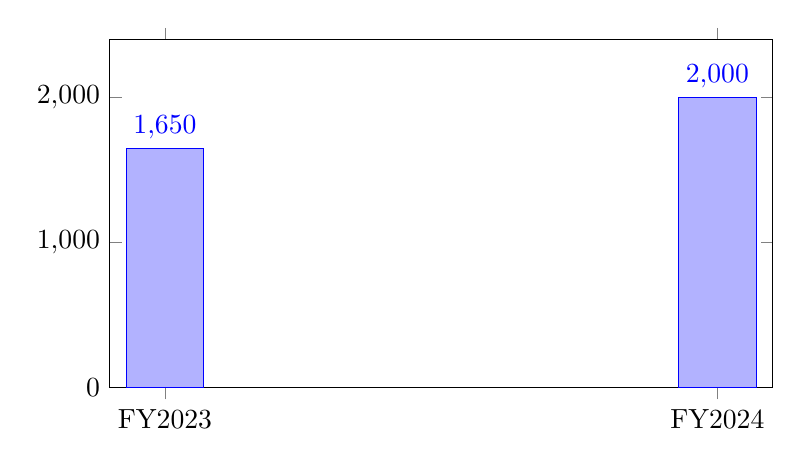
\begin{tikzpicture}
\begin{axis}[
    ybar, width=10cm, height=6cm,
    symbolic x coords={FY2023, FY2024},
    xtick=data, ymin=0, ymax=2400,
    nodes near coords, bar width=28pt,
]
\addplot coordinates {(FY2023, 1650) (FY2024, 2000)};
\end{axis}
\end{tikzpicture}

\end{document}
